\pdfminorversion=4
\documentclass{beamer}
%%%%%%%%%%%%%%%%%%%%%%%%%%%%%%%%%%%%%%%%%%%%%%%%%%%%%%%%%%%%%
\usepackage{amssymb}
\usepackage{mathpazo}
\usepackage{multimedia}
\usepackage{amsfonts}
\usepackage{amsmath}
\usepackage{hyperref}
\usepackage{listings}
\lstset{language=Matlab,commentstyle=\color{mygreen}} 

\setcounter{MaxMatrixCols}{10}


\hypersetup{
colorlinks = true,
allcolors = blue,
}
\definecolor{mygreen}{rgb}{0,0.6,0}
\newtheorem{prop}{Proposition}
%\newtheorem{corollary}{Corollary}

\setbeamertemplate{footline}[frame number]
\setbeamertemplate{navigation symbols}{}
\setbeamertemplate{mini frames}{}
\setbeamertemplate{itemize item}[ball]
\setbeamertemplate{itemize subitem}[ball]
\setbeamercovered{invisible}

%------------- NEW COMMANDS ----------------------------------------%
\newcommand{\eps}{\varepsilon}
\newcommand{\E}{\mathbb{E}}
\newcommand{\I}{\mathbb{I}}

\newcommand{\beginbackup}{
   \newcounter{framenumbervorappendix}
   \setcounter{framenumbervorappendix}{\value{framenumber}}
}
\newcommand{\backupend}{
   \addtocounter{framenumbervorappendix}{-\value{framenumber}}
   \addtocounter{framenumber}{\value{framenumbervorappendix}} 
}
\renewcommand{\baselinestretch}{1.2}
\small\normalsize
\subtitle{A simple two-period model}
\institute[Universities Here and There]{University of Birmingham}

%\input{tcilatex}

\begin{document}

\title{Advanced Numerical Methods}
\subtitle{Solving DSGE Models with Dynare, Part 3}
\author{Alessandro~Di Nola}
\date{}

\begin{frame}
\titlepage
\end{frame}

%\section{Notation}

%TCIMACRO{\TeXButton{BeginFrame}{\begin{frame}}}%
%BeginExpansion
\begin{frame}%
%EndExpansion
\frametitle{Outline}

\begin{itemize}
\item Steady-state computation
\medskip
\item Incorporating Dynare in matlab programs
\medskip
\item Blanchard-Kahn conditions and indeterminacy
\medskip
%\item How to extract solution matrices and run your own simulations

\item Computation of moments

\begin{itemize}
\item Theoretical moments

\item Moments based on stochastic simulations
\end{itemize}

%\item Perturbation and the effect of uncertainty on the solution

%\item Higher order perturbation
\end{itemize}

\end{frame}
%%%%%%%%%%%%%%%%%%%%%%%%%%%%%%%%%%%%%%%%%%%%%%

\begin{frame}[fragile]
\frametitle{Steady-state computation}
\framesubtitle{Basic}
\begin{itemize}
\item Hardest part of Dynare is to solve for steady state.
\item Solving for the steady state $ \equiv $ solving a system of \textcolor{blue}{nonlinear} equations.
\pause 
\item Simplest way: give initial guesses using ``initval'' command.
\item Then Dynare starts a numerical solver to find the steady-state. 
\begin{verbatim}
initval;
c = 0.75;
k = 3;
z = 1;
e = 0;
end;
steady;
\end{verbatim}

\end{itemize}

\end{frame}
%%%%%%%%%%%%%%%%%%%%%%%%%%%%%%%%%%%%%%%%%%%%%%%%%%

\begin{frame}
\frametitle{Steady-state computation}
\framesubtitle{Basic}
\begin{itemize}
	\item Use \textcolor{blue}{economic intuition} to come up with good initial guesses!
	\begin{itemize}
		\item E.g. in the RBC model, $ I<C<Y<K $.
	\end{itemize}
    \pause 
	\item Unfortunately, with more complicated models not so easy to find good guesses. \item $ \rightarrow $ Basic method does not perform very well in practice.
\end{itemize}
\end{frame}
%%%%%%%%%%%%%%%%%%%%%%%%%%%%%%%%%%%%%%%%%%%%%%%%%%

\begin{frame}
\frametitle{Steady-state computation}
\framesubtitle{Advanced}
\begin{itemize}
	\item Three (advanced) methods:
	\begin{enumerate}
		\item Compute the steady state \textcolor{blue}{analytically} and provide it to Dynare using
		the \texttt{steady\_state\_model} command.
		\pause
		\item Compute the steady state \textcolor{red}{numerically} in Matlab and pass your numerical solution as an educated guess to Dynare.
		\pause
		\item Use an explicit \textcolor{red}{steady state file}, which requires that you follow strict programming rules.
	\end{enumerate}
    \pause 
    \item \textcolor{red}{TIP}: method 2 works well in practice.
\end{itemize}
\end{frame}
%%%%%%%%%%%%%%%%%%%%%%%%%%%%%%%%%%%%%%%%%%%%%%%%%%

\begin{frame}[fragile]
\frametitle{Steady-state computation: Method 1}
\framesubtitle{Advanced}
\small 
\begin{itemize}
	\item Stochastic growth model seen in Lectures 1/2/3.
	
	\item Deterministic steady-state:%
	\begin{equation*}
	\bar{k}=\left( \frac{\alpha \beta \bar{z}}{1-\beta \left( 1-\delta \right) }\right) ^{%
		\frac{1}{1-\alpha }},\ \bar{c}=\bar{z}\bar{k}^{\alpha }-\delta \bar{k}\text{, }\bar{z}=1
	\end{equation*}
	\item Steady-state block in Dynare:
	\begin{verbatim}
	steady_state_model;
	z_ss = 1;
	k_ss = (alpha*z_ss/(1/beta-1+delta))^(1/(1-alpha));
	c_ss = z_ss*k_ss^alpha - delta*k_ss;
	y_ss = z_ss*k_ss^alpha;
	c = log(c_ss); k = log(k_ss);
	y = log(y_ss); z = log(z_ss);
	end;
	steady;
	\end{verbatim}
	
\end{itemize}
\end{frame}
%%%%%%%%%%%%%%%%%%%%%%%%%%%%%%%%%%%%%%%%%%%%%%%%%%

\begin{frame}[fragile]
\frametitle{Steady-state computation: Method 1}
\framesubtitle{Advanced}
\small 
\begin{itemize}
	\item You can find the necessary files to implement this method on ILIAS. Go to \texttt{Codes}, \texttt{Dynare:steady state}.
	\begin{itemize}
		\item Relevant files are \texttt{main1.m} and \texttt{growth1.mod}.
	\end{itemize}
\end{itemize}
\end{frame}
%%%%%%%%%%%%%%%%%%%%%%%%%%%%%%%%%%%%%%%%%%%%%%%%%%


\begin{frame}[fragile]
\frametitle{Steady-state computation: Method 2}
\framesubtitle{Advanced}
\small 
\begin{itemize}
	\item For some models, not easy to find steady state analytically.
	\item Compute numerically s.s. in Matlab.
	\begin{itemize}
		\item Use all the flexibility of Matlab programming environment.
	\end{itemize}
    \item Save your numerical results in a \texttt{*.mat} file:
	\begin{verbatim}
	save paramfile z_ss k_ss c_ss y_ss
	\end{verbatim}
	\item Load \texttt{*.mat} file in Dynare. \textbf{Declare ss values as extra parameters}.
	\begin{verbatim}
	parameters alpha, beta, delta, sigma, rho, sigmaeps, 
	z_ss, k_ss, c_ss, y_ss;  
	load paramfile
	set_param_value('z_ss',z_ss)
	set_param_value('k_ss',k_ss)
	....
	\end{verbatim}
\end{itemize}
\end{frame}
%%%%%%%%%%%%%%%%%%%%%%%%%%%%%%%%%%%%%%%%%%%%%%%%%%

\begin{frame}[fragile]
\frametitle{Steady-state computation: Method 2}
\framesubtitle{Advanced}
\small 
\begin{itemize}
	\item Use imported values \texttt{z\_ss}, \texttt{k\_ss}, \texttt{c\_ss}, \texttt{y\_ss} as ``educated'' initial conditions in the initval block.
	\begin{verbatim}
	initval;
	c = log(c_ss);
	k = log(k_ss);
	y = log(y_ss);
	z = log(z_ss);
	end;
	steady;
	\end{verbatim}
\end{itemize}
\end{frame}
%%%%%%%%%%%%%%%%%%%%%%%%%%%%%%%%%%%%%%%%%%%%%%%%%%

\begin{frame}[fragile]
\frametitle{Steady-state computation: Method 2}
\framesubtitle{Advanced}
\small 
\begin{itemize}
	\item How to compute numerically steady state in Matlab?
	\item Matlab has several \textcolor{blue}{nonlinear solvers}.
	\item In practice, \texttt{fsolve} performs well. 
\end{itemize}
\end{frame}
%%%%%%%%%%%%%%%%%%%%%%%%%%%%%%%%%%%%%%%%%%%%%%%%%%

\begin{frame}[fragile]
\frametitle{Steady-state computation: Method 2}
\framesubtitle{Advanced}
\small 
\begin{itemize}
	\item Write function with nonlinear equations that define the steady state.
	\begin{verbatim}
	function F = ss_eq(x,params)
	\end{verbatim}
	\item Inputs: $ n \times 1 $ vector \texttt{x}, with $ n $ equal to \# endo variables.
	\item Anything else in \texttt{params}. 
	\item Ouput: vector-valued function $ F:R^{n}\rightarrow R^{n}$.
	\item Each element of vector $ F $ is a steady state equation.
	\item Note: you don't have to follow \textit{exactly} this structure.
	\begin{itemize}
		\item E.g., can add other variables as inputs or outputs to the function.
	\end{itemize}
\end{itemize}
\end{frame}
%%%%%%%%%%%%%%%%%%%%%%%%%%%%%%%%%%%%%%%%%%%%%%%%%%

\begin{frame}[fragile]
\frametitle{Steady-state computation: Method 2}
\framesubtitle{Advanced}
\small 

	\begin{verbatim}
	function F = ss_eq(x,beta,alpha,delta)
	c = x(1);
	k = x(2);
	y = x(3);
	z = x(4);
	% Pre-allocate vector F(x)
	F = zeros(4,1);
	% Type your steady-state relationships.
	F(1) = c - y -delta*k;                       % res.constr. (1)
	F(2) = 1-beta*(alpha*z*k^(alpha-1)+1-delta); % Euler       (2)
	F(3) = y - z*k^alpha;                        % prod. f.    (3)
	F(4) = z - 1;                                % AR1         (4)
	end
	\end{verbatim}
\end{frame}
%%%%%%%%%%%%%%%%%%%%%%%%%%%%%%%%%%%%%%%%%%%%%%%%%%

\begin{frame}[fragile]
\frametitle{Steady-state computation: Method 2}
\framesubtitle{Advanced}
\small 

\begin{itemize}
	\item \textcolor{red}{TIP}: it's a good idea to simplify as much as you can manually.
	\begin{itemize}
		\item For example, type this:
		
		\begin{equation*}
		1-\beta*(\alpha*z*k^{(\alpha-1)} + 1 -\delta) = 0
		\end{equation*}
		
		\item instead of:
		
		\begin{equation*}
		c^{-\sigma}-\beta*c^{-\sigma}*(\alpha*z*k^{(\alpha-1)} + 1 -\delta) = 0
		\end{equation*}
	\end{itemize}
	\pause 
	\item Become familiar with \texttt{fsolve} options.
	\begin{itemize}
		\item Tighten tolerance criteria: \texttt{FunctionTolerance} and \texttt{TolX}.
		\item Try different algorithms: \texttt{trust-region-dogleg} (default), \texttt{trust-region}, and \texttt{levenberg-marquardt}.
	\end{itemize}
	
\end{itemize}

\end{frame}
%%%%%%%%%%%%%%%%%%%%%%%%%%%%%%%%%%%%%%%%%%%%%%%%%%

\begin{frame}[fragile]
\frametitle{Steady-state computation: Method 2}
\framesubtitle{Advanced}
\small 
\begin{itemize}
	\item You can find the necessary files to implement this method on ILIAS. Go to \texttt{Codes}, \texttt{Dynare:steady state}.
	\begin{itemize}
		\item Relevant files are \texttt{main2.m} and \texttt{growth2.mod}.
	\end{itemize}
\end{itemize}
\end{frame}
%%%%%%%%%%%%%%%%%%%%%%%%%%%%%%%%%%%%%%%%%%%%%%%%%%

\begin{frame}[fragile]
\frametitle{Steady-state computation: Method 3}
\framesubtitle{Advanced}
\small 

\begin{itemize}
	\item Write a Matlab ``steady state function'' following Dynare \textcolor{red}{strict rules}.
	\item If the mod file is named \texttt{myfile.mod}, then steady state file \textbf{must} be called \texttt{myfile\_steadystate.m}.
	\item Dynare saves parameter values in structure \texttt{M\_}.
	\item In your ss file, you \textbf{must} read the parameters from \texttt{M\_}. You \textbf{cannot} pass the parameter values as extra inputs to the function.
	\item After solving for the ss, you \textbf{must} store the results in vector \texttt{ys}. 
	\item \texttt{ys} \textbf{must} be declared both as an input and as an output.
	\item You \textbf{must} include an exit flag, called ``check'', as a second output.
	\item You \textbf{must} include \texttt{exe} as a second input.
\end{itemize}

\end{frame}
%%%%%%%%%%%%%%%%%%%%%%%%%%%%%%%%%%%%%%%%%%%%%%%%%%

\begin{frame}[fragile]
\frametitle{Steady-state computation: Method 3}
\framesubtitle{Advanced}
\small 
\begin{itemize}
	\item Suppose your mod file is named \texttt{growth3.mod}.
\end{itemize}
\begin{verbatim}
function [ys,check] = growth3_steadystate(ys,exe)
global M_
alpha    = M_.params(1);  
beta     = M_.params(2);  
delta    = M_.params(3); 
% Solve for steady-state
% Get c_ss, k_ss, y_ss and z_ss
.......
check = 0;

ys = [log(c_ss);log(k_ss);log(y_ss);log(z_ss)];

end
\end{verbatim}
\end{frame}
%%%%%%%%%%%%%%%%%%%%%%%%%%%%%%%%%%%%%%%%%%%%%%%%%%

\begin{frame}[fragile]
\frametitle{Steady-state computation: Method 3}
\framesubtitle{Advanced}
\small 
\begin{itemize}
	\item You can find the necessary files to implement this method on ILIAS. Go to \texttt{Codes}, \texttt{Dynare:steady state}.
	\begin{itemize}
		\item Relevant files are \texttt{main3.m}, \texttt{growth3.mod} and \texttt{growth3\_steadystate.mod}.
	\end{itemize}
\end{itemize}
\end{frame}
%%%%%%%%%%%%%%%%%%%%%%%%%%%%%%%%%%%%%%%%%%%%%%%%%%


\begin{frame}
\frametitle{Dynare in matlab programs}

\begin{itemize}
\item Dynare can be nested into Matlab programs.

\item Already seen this in Lecture 3 - looping over parameters.

\item But is much more general and useful for:

\begin{itemize}
\item Passing to Dynare steady-state values computed beforehand in Matlab.

\item Nesting mod file inside an estimation routine written in Matlab (GMM,
IRF matching, etc.).
\end{itemize}

\item \textcolor{red}{Warning}: Dynare clears the memory before starting (so if there are
some matlab calculations before, the results will be cancelled). 
\begin{itemize}
	\item To avoid this use:
	\texttt{dynare myfile.mod noclearall}.
\end{itemize}

\end{itemize}

\end{frame}
%%%%%%%%%%%%%%%%%%%%%%%%%%%%%%%%%%%%%%%%%%%%%%

\begin{frame}%
%EndExpansion
\frametitle{Dynare in matlab programs}

\begin{itemize}
\item Suppose you want to produce moments or IRFs for different parameter configurations.
\medskip
\begin{itemize}
	\item How a change in $ \rho $ (persistence of TFP shocks) affects the dynamic response of model endogenous variables?
	\medskip
	\item How a change in CRRA $ \sigma $ affects the relative standard deviation of consumption w.r.t. output?
\end{itemize}

\end{itemize}

\end{frame}
%%%%%%%%%%%%%%%%%%%%%%%%%%%%%%%%%%%%%%%%%%%%%%

\begin{frame}[fragile]
%EndExpansion
\frametitle{Dynare in matlab programs: IRFs}

\begin{itemize}
	\item IRFs of $ c,k $ for  $ \rho \in \{0.5,0.95\}$
\begin{lstlisting}[frame=single]
rho_vec = [0.5 0.95];
c_irf = zeros(T_irf,2);
k_irf = zeros(T_irf,2);
% Start loop
for i = 1:2	
  rho = rho_vec(i);
  save paramfile.mat rho
  dynare growth.mod noclearall
  c_irf(:,i) = c_e;
  k_irf(:,i) = k_e;
end
\end{lstlisting}
	
\end{itemize}

\end{frame}
%%%%%%%%%%%%%%%%%%%%%%%%%%%%%%%%%%%%%%%%%%%%%%

\begin{frame}[fragile]
%EndExpansion
\frametitle{Dynare in matlab programs}

\begin{figure}
	\centering
	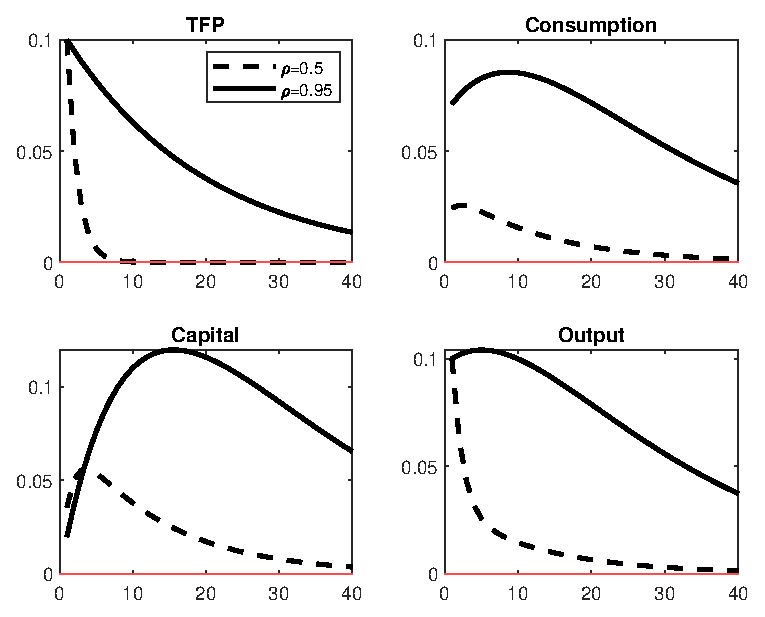
\includegraphics[width=0.7\linewidth]{../figs/irfs_rho}
	
\end{figure}
IRF of $ z,c,k,y $ to a 0.1 positive shock to $ z $, for $ \rho=0.5 $ (dashed line) and $ \rho=0.95 $ (solid line).

\end{frame}
%%%%%%%%%%%%%%%%%%%%%%%%%%%%%%%%%%%%%%%%%%%%%%

\begin{frame}[fragile]
\frametitle{Dynare in matlab programs: Moments}

\begin{itemize}
\item Relative stdev. of $ c $ for  $ \sigma \in \left[ 0.5,\dots,3\right] $
\begin{lstlisting}[frame=single]
sigma_vec = linspace(0.5,3,np);
c_stdev = zeros(np,1);
% Start loop
for i = 1:np
sigma = sigma_vec(i);
save paramfile.mat sigma
dynare stoch_growth2.mod noclearall  
c_stdev(i) = sqrt(oo_.var(c_pos,c_pos))/...
sqrt(oo_.var(y_pos,y_pos));
end
\end{lstlisting}
	
\end{itemize}

\end{frame}
%%%%%%%%%%%%%%%%%%%%%%%%%%%%%%%%%%%%%%%%%%%%%%

\begin{frame}[fragile]
\frametitle{Dynare in matlab programs: Moments}

\begin{figure}
	\centering
	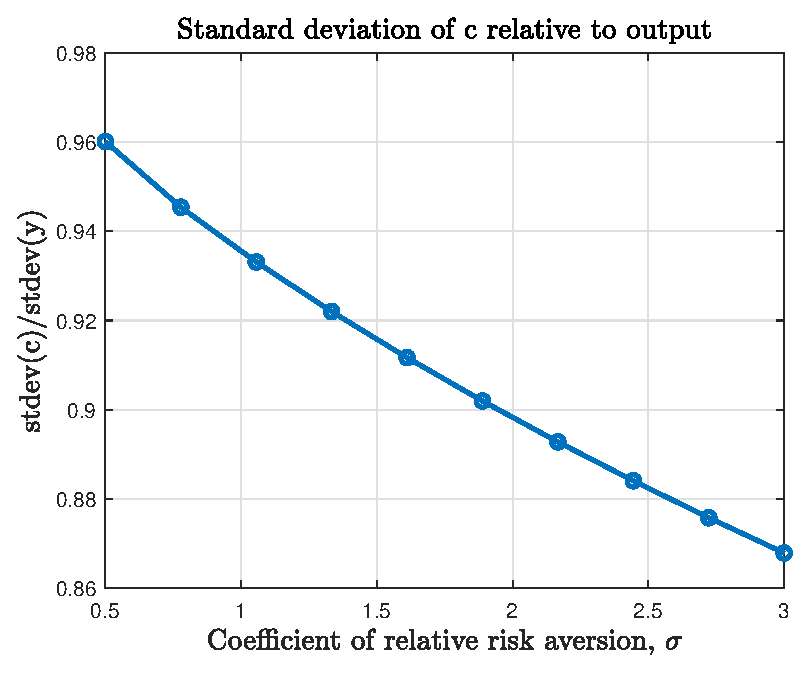
\includegraphics[width=0.7\linewidth]{../figs/stdev_c_y}
	
\end{figure}

\end{frame}
%%%%%%%%%%%%%%%%%%%%%%%%%%%%%%%%%%%%%%%%%%%%%%

\begin{frame}
\frametitle{Blanchard-Kahn conditions in Dynare}

\begin{itemize}
	\item Recall Blanchard-Kahn conditions seen in Lecture 2:
	
	\begin{itemize}
		\item Number of unstable eigenvalues = number of forward-looking variables $ \implies $ \textcolor{blue}{unique solution}.
		\item Number of unstable eigenvalues $ > $ number of forward-looking variables $ \implies $ \textcolor{red}{no solution}.
		\item Number of unstable eigenvalues $ < $ number of forward-looking variables $ \implies $ \textcolor{red}{indeterminacy}.
	\end{itemize}
	
	\item How does this work in Dynare?
	\item Simple example based on the New-Keynesian model.
	\begin{itemize}
		\item Dynare error message 1: Example with indeterminacy.
		
		\item Dynare error message 2: Example with no solution.
	\end{itemize}
\end{itemize}

\end{frame}
%%%%%%%%%%%%%%%%%%%%%%%%%%%%%%%%%%%%%%%%%%%%%%


\begin{frame}
\frametitle{New-Keynesian model}

\begin{itemize}
\item Consider plain vanilla NK model:
\begin{align*}
x_{t} &= \E_{t}x_{t+1} -\frac{1}{\sigma} (i_{t}-\E_{t}\pi_{t+1}-r) \\
\pi_{t} &= \beta \E_{t}\pi_{t+1}+\kappa x_{t} \\
i_{t} &= r+\textcolor{red}{\delta} \pi_{t}+v_{t} \\
v_{t} &= \rho_{v}v_{t-1}+\eps_{t}, \ \eps_{t}\sim N(0,1).
\end{align*}
where $ x_{t} $ is output gap, $ \pi_{t} $ is inflation rate, $ i_{t} $ is nominal interest rate and $ v_{t} $ is a policy shock.
\item \underline{Key parameter}: $ \textcolor{red}{\delta} $ measures how strongly the central bank reacts to inflation.

\end{itemize}

\end{frame}
%%%%%%%%%%%%%%%%%%%%%%%%%%%%%%%%%%%%%%%%%%%%%%

\begin{frame}
\frametitle{New-Keynesian model: Unique Equilibrium?}

\begin{itemize}
	\item The model has a unique stationary solution iff the number of eigenvalues larger than one (in modulus) is equal to the number of forward-looking variables.
	\item What are the forward-looking variables in this model?
	\pause 
	\item Nominal interest rate is static (indeed, it can be eliminated from the system).
	\item The only predetermined variable is the policy shock $ v_{t} $ (exogenous state variable).
	\pause
	\item Inflation $ \pi_{t} $ and output gap $ x_{t} $ are forward-looking.
	
	\item Unique equilibrium requires \textbf{two} unstable eigenvalues.
	
\end{itemize}

\end{frame}
%%%%%%%%%%%%%%%%%%%%%%%%%%%%%%%%%%%%%%%%%%%%%%

\begin{frame}[fragile]
\frametitle{New-Keynesian model}

\begin{itemize}
	\item Write down the model in Dynare:
	\begin{verbatim}
	model(linear); 
	#kappa = (sigma+eta)*((1-omega)*(1-beta*omega)/omega);
	// (1) IS curve
	x = x(+1) -(1/sigma)*(i-pi(+1)-r);
	// (2) NK Philips curve
	pi = beta*pi(+1)+kappa*x;
	// (3) Taylor rule
	i = r+delta*pi+v;
	// (4) Policy shock
	v = rho_v*v(-1)+e;
	end;
	\end{verbatim}
\end{itemize}

\end{frame}
%%%%%%%%%%%%%%%%%%%%%%%%%%%%%%%%%%%%%%%%%%%%%%

\begin{frame}[fragile]
\frametitle{New-Keynesian model}

\begin{itemize}
	\item Suppose we set $ \delta = 0.5$. Any problem?
	\pause
	\item Suppose we set $ \rho_{v} = 1.5$. Any problem?
	\pause 
	\item Blanchard-Kahn conditions for unique equilibrium require: $ \delta>1$ and $ \rho_{v}\in(-1,1)$. 
	\item The restriction $ \delta>1$ is known as the \textit{Taylor principle}.
\end{itemize}

\end{frame}
%%%%%%%%%%%%%%%%%%%%%%%%%%%%%%%%%%%%%%%%%%%%%%

\begin{frame}[fragile]
\frametitle{New-Keynesian model: Indeterminacy}

\begin{itemize}
	\item Set $ \delta = 0.5$. Nominal interest rate does not respond strongly enough to inflation $ \implies $ multiple equilibria/indeterminacy.
	\item If you try to run Dynare under such parametrization, you'll get:
\end{itemize}
\begin{figure}
	\centering
	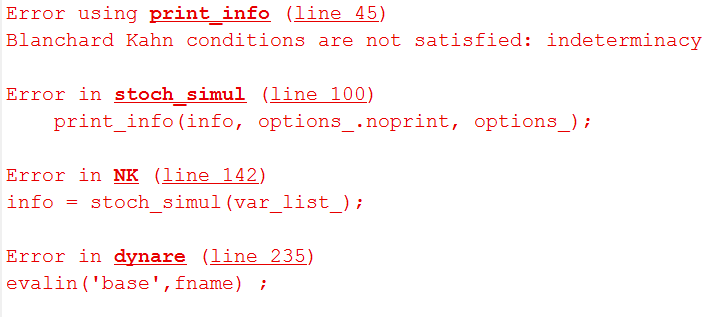
\includegraphics[width=0.8\linewidth]{../figs/dynare_error_indet}
	
\end{figure}

\end{frame}
%%%%%%%%%%%%%%%%%%%%%%%%%%%%%%%%%%%%%%%%%%%%%%

\begin{frame}[fragile]
\frametitle{New-Keynesian model: No solution}

\begin{itemize}
	\item Set $ \rho_{v} = 1.5$. The AR(1) process for policy shock is ``explosive''.
	\item If you try to run Dynare under such parametrization, you'll get:
\end{itemize}
\begin{figure}
	\centering
	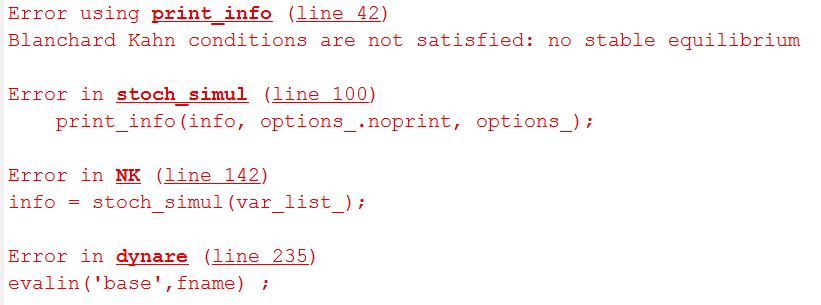
\includegraphics[width=0.8\linewidth]{../figs/dynare_error_nosolution}
	
\end{figure}

\end{frame}
%%%%%%%%%%%%%%%%%%%%%%%%%%%%%%%%%%%%%%%%%%%%%%

\begin{frame}[fragile]
\frametitle{New-Keynesian model: Unique equilibrium}

\begin{itemize}
	\item Set $ \delta=1.5 $ and $ \rho_{v} = 0.5$. 
	\item Dynare verifies that BK conditions are satisfied and proceeds with solution.
\end{itemize}
\begin{figure}
	\centering
	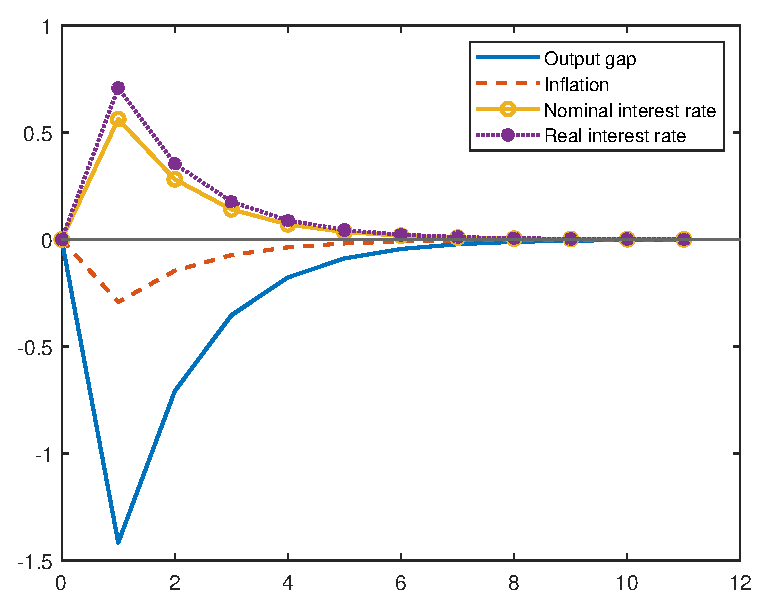
\includegraphics[width=0.7\linewidth]{../figs/nk_graph}
	
\end{figure}

\end{frame}
%%%%%%%%%%%%%%%%%%%%%%%%%%%%%%%%%%%%%%%%%%%%%%


\begin{frame}[fragile]
\frametitle{Correlated shocks}

\begin{itemize}
\item In simple example with growth model $\implies $ only one exogenous
shock $\varepsilon _{t}$ to technology.

\item \textbf{Assuming \texttt{sig\_eps} denotes the standard deviation}, we can specify the ``shock block'' in two equivalent ways:
\end{itemize}

\begin{columns}[c]
	
	\column{.45\textwidth} % Left column and width
	\begin{verbatim}
	shocks;
	var e = sig_eps^2;
	end;
	\end{verbatim}
	
	\column{.5\textwidth} % Right column and width
	\begin{verbatim}
	shocks;
	var e; stderr sig_eps;
	end;
	\end{verbatim}

\end{columns}

\end{frame}
%%%%%%%%%%%%%%%%%%%%%%%%%%%%%%%%%%%%%%%%%%%%%%

\begin{frame}
\frametitle{Correlated shocks, cont'd}
	\begin{itemize}
		\item Example with two correlated shocks $\left( a_{t},z_{t}\right) $:
		\begin{align*}
	    a_{t} &= \rho_{a}a_{t-1}+\eps_{at}, \\
	    z_{t} &= \rho_{z}z_{t-1}+\eps_{zt}
		\end{align*}
		where 
		\begin{equation*}
		\begin{bmatrix}
		\eps_{at} \\ 
		\eps_{zt}%
		\end{bmatrix}%
		\sim N\left( 0,\Sigma \right).
		\end{equation*}
		
		\item The \textcolor{blue}{variance-covariance matrix} is:
		\begin{equation*}
		\Sigma =%
		\begin{bmatrix}
		\sigma _{a}^{2} & \sigma _{a,z}^{2} \\ 
		\sigma _{a,z}^{2} & \sigma _{z }^{2}%
		\end{bmatrix}%
		\end{equation*}
		
		\item Note: $COV(\eps_{at},\eps_{zt})\equiv\sigma _{a,z}^{2}=\phi \cdot \sigma
		_{a}\cdot \sigma_{z}$, where $ \phi $ is the \textcolor{red}{correlation} coefficient.
	\end{itemize}

\end{frame}
%%%%%%%%%%%%%%%%%%%%%%%%%%%%%%%%%%%%%%%%%%%%%%

\begin{frame}[fragile]
\frametitle{Correlated shocks, cont'd}

We have again two equivalent ways to specify the ``shocks block'':

\small 
\begin{columns}[c]
	
	\column{.45\textwidth} % Left column and width
	\begin{verbatim}
	shocks;
	var ea = sig_a^2;
	var ez = sig_z^2;
	var ea,ez = phi*sig_a*sig_z;
	end;
	\end{verbatim}
	
	\column{.5\textwidth} % Right column and width
	\begin{verbatim}
	shocks;
	var ea; stderr sig_a;
	var ez; stderr sig_z;
	var ea,ez = phi*sig_a*sig_z;
	end;
	\end{verbatim}
	
\end{columns}

\end{frame}
%%%%%%%%%%%%%%%%%%%%%%%%%%%%%%%%%%%%%%%%%%%%%%

\begin{frame}
\frametitle{Theoretical vs Simulated Moments}
\small 
\begin{itemize}
	\item Suppose we have a solution of a DSGE model.
	\item How to compute moments (i.e. variance, autocorrelation, etc.) of variables of interest?
	\pause 
	\item Consider simple AR(1) model:
	\begin{equation}\label{eq:ar1}
	y_{t} = ay_{t-1}+\eps_{t}
	\end{equation}
	where $ \eps_{t} $ is IID shock with mean 0 and variance $ \sigma^{2} $.
	\item How to compute, e.g., $ var(y_{t}) \equiv \gamma_{0} $?
	\item One way: \textcolor{blue}{simulation}
	\begin{itemize}
		\item Draw a sequence of shocks $ \left\lbrace \eps_{t} \right\rbrace_{t=0}^{T}  $, with $ T $ large.
		\item Generate simulated series $ \{y_{t} \}_{t=0}^{T} $ iterating on (\ref{eq:ar1}), starting from an arbitrary $ y_{0} $.
	\end{itemize}
\end{itemize}
\end{frame}
%%%%%%%%%%%%%%%%%%%%%%%%%%%%%%%%%%%%%%%%%%%%%%%%%%

\begin{frame}
\frametitle{Theoretical vs Simulated Moments}
\framesubtitle{Simulation, cont'd}
\small 
\begin{itemize}
	\item Given simulated series $ \{y_{t} \}_{t=0}^{T} $, one can compute variance and autocovariances of $ y $ as follows:
	
	\begin{align*}
	\hat{\gamma}_{0} &= \left(\frac{1}{T} \right)\sum_{t=1}^{T}(y_{t}-\bar{y})^{2} \\
	\hat{\gamma}_{j} &= \left(\frac{1}{T} \right)\sum_{t=j+1}^{T}(y_{t}-\bar{y})(y_{t-j}-\bar{y})^{2}
	\end{align*}
	where $ \bar{y} $ is the sample average.
	
\end{itemize}
\end{frame}
%%%%%%%%%%%%%%%%%%%%%%%%%%%%%%%%%%%%%%%%%%%%%%%%%%

\begin{frame}
\frametitle{Theoretical vs Simulated Moments}
\framesubtitle{Theoretical Moments}
\small 
\begin{itemize}
	\item However, for linear models, the computation of relevant moments can be done also analytically.
	\item Well known results for (stationary) AR(1) models:
	
	\begin{align*}
	Var(y_{t}) \equiv \gamma_{0} &= \frac{\sigma^{2}}{1-a^{2}} \\
	Cov(y_{t},y_{t-j}) \equiv \gamma_{j} &= a^{j}\frac{\sigma^{2}}{1-a^{2}}
	\end{align*}
	for $ j=1,2,\dots $
	
	\item Of course a law of large numbers will typically ensure that
	$$ \hat{\gamma}_{0} \rightarrow \gamma_{0}, \ \hat{\gamma}_{j} \rightarrow \gamma_{j} \text{ as } T \rightarrow \infty$$
\end{itemize}
\end{frame}
%%%%%%%%%%%%%%%%%%%%%%%%%%%%%%%%%%%%%%%%%%%%%%%%%%

\begin{frame}
\frametitle{Theoretical Moments}
\framesubtitle{How Dynare computes them}
\small 
\begin{itemize}
	\item Consider multivariate case $ n>1 $.
	\item DSGE solution can be mapped into a VAR(1):
	\begin{equation*}
	y_{t}=Ay_{t-1}+\varepsilon _{t}
	\end{equation*}%
	where $y_{t}$ is the vector of endogenous variables and $\varepsilon _{t}$
	is vector of exogenous shocks. $A$ is a $n\times n$ matrix and $\varepsilon
	_{t}\sim N\left( 0,\Sigma \right) $ where $\Sigma $ is the var-cov matrix of 
	$\varepsilon _{t}$. 
	\item Let $\Gamma _{0}=\E\left( y_{t}y_{t}^{\prime }\right) $ denote the var-cov
	matrix of $y_{t}$ and $\Gamma _{j}=\E\left( y_{t}y_{t-j}^{\prime }\right) $
	denote the $j$th order autocovariance matrix.
	
\end{itemize}
\end{frame}
%%%%%%%%%%%%%%%%%%%%%%%%%%%%%%%%%%%%%%%%%%%%%%%%%%

\begin{frame}
\frametitle{Theoretical Moments}
\framesubtitle{How Dynare computes them}
\small 
\begin{itemize}
	\item (Contemporaneous) variance-covariance matrix of $ y_{t} $, $\Gamma _{0}$:
	\begin{align*}
		\Gamma _{0} &=\E\left( y_{t}y_{t}^{\prime }\right)  \\
		&=\E\left[ \left( Ay_{t-1}+\varepsilon _{t}\right) \left(
		Ay_{t-1}+\varepsilon _{t}\right) ^{\prime }\right]  \\
		&=A\E\left( y_{t-1}y_{t-1}^{\prime }\right) A^{\prime }+\E\left( \varepsilon
		_{t}\varepsilon _{t}^{\prime }\right)  \\
		&=A\Gamma _{0}A^{\prime }+\Sigma 
	\end{align*}
	\item Hence we found that 
	\begin{equation*}
	\boxed{\Gamma _{0}=A\Gamma _{0}A^{\prime }+\Sigma}
	\end{equation*}%
	\item How do we solve for $\Gamma _{0}$? 
\end{itemize}
\end{frame}
%%%%%%%%%%%%%%%%%%%%%%%%%%%%%%%%%%%%%%%%%%%%%%%%%%

\begin{frame}
\frametitle{Theoretical Moments}
\framesubtitle{How Dynare computes them}
\label{kronBack}
\small 
\begin{itemize}
	\item Use \textcolor{blue}{vec}-torization operator to simplify $\Gamma _{0}=A\Gamma _{0}A^{\prime }+\Sigma$.
	\item Recall that
	\begin{align*}
	vec\left( A+B\right) &= vec(A) + vec(B) \\
	vec\left( ABC\right) &=\left( C^{\prime }\otimes A\right) vec\left( B\right)
	\end{align*}
	\item it follows that
	\begin{align*}
	vec\left( \Gamma _{0}\right)  &=vec\left( A\Gamma _{0}A^{\prime }\right)
	+vec\left( \Sigma \right)  \\
	vec\left( \Gamma _{0}\right)  &=\left( A\otimes A\right) vec\left( \Gamma
	_{0}\right) +vec\left( \Sigma \right) 
	\end{align*}
	\item Hence
	\begin{equation*}
	vec\left( \Gamma _{0}\right) =\left[ I-\left( A\otimes A\right) \right]
	^{-1}vec\left( \Sigma \right).
	\end{equation*}%
	where $I$ has dimension $n^{2}\times n^{2}$. \hyperlink{kron}{\beamerbutton{Math}}
\end{itemize}
\end{frame}
%%%%%%%%%%%%%%%%%%%%%%%%%%%%%%%%%%%%%%%%%%%%%%%%%%

\begin{frame}
\frametitle{Theoretical Moments}
\framesubtitle{How Dynare computes them}
\small 
\begin{itemize}
	\item Likewise, for the autocovariance%
	\begin{align*}
		\Gamma _{1} &=\E\left( y_{t}y_{t-1}^{\prime }\right)  \\
		&=\E\left[ \left( Ay_{t-1}+\varepsilon _{t}\right) y_{t-1}^{\prime }\right] 
		\\
		&=A\E\left( y_{t-1}y_{t-1}^{\prime }\right) +\E\left( \varepsilon
		_{t}y_{t-1}^{\prime }\right)  \\
		&=A\Gamma _{0}
	\end{align*}%
	and in general%
	\begin{align*}
		\Gamma _{j} &=A\Gamma _{j-1} \\
		&=A^{j}\Gamma _{0}
	\end{align*}%
	for $j=1,2,\ldots $
\end{itemize}
\end{frame}
%%%%%%%%%%%%%%%%%%%%%%%%%%%%%%%%%%%%%%%%%%%%%%%%%%

\begin{frame}
\frametitle{Theoretical Moments}
\framesubtitle{How Dynare computes them}
\small 
\begin{itemize}
	\item Recall DSGE solution:
	\begin{align*}
		s_{t} &=\Pi s_{t-1}+W\varepsilon _{t}, \eps_{t} \sim N(0,\Sigma_{\eps}) \\
		u_{t} &=Us_{t}
	\end{align*}%
	Clearly, to fit the model into VAR(1) notation, set 
	\begin{align*}
		A &=\Pi  \\
		\Sigma  &=W\Sigma _{\varepsilon }W^{\prime }
	\end{align*}
	\item In our stochastic growth model $\Sigma _{\varepsilon }$ is simply a scalar $%
	\sigma _{e}^{2}$ and $W=\left[ 0,1\right] ^{\prime }$, so 
	\begin{equation*}
	\Sigma =%
	\begin{bmatrix}
	0 \\ 
	1%
	\end{bmatrix}%
	\sigma _{\varepsilon }^{2}%
	\begin{bmatrix}
	0 & 1%
	\end{bmatrix}%
	=%
	\begin{bmatrix}
	0 & 0 \\ 
	0 & \sigma _{\varepsilon }^{2}%
	\end{bmatrix}%
	\end{equation*}%
	
\end{itemize}
\end{frame}
%%%%%%%%%%%%%%%%%%%%%%%%%%%%%%%%%%%%%%%%%%%%%%%%%%

\begin{frame}
\frametitle{Theoretical Moments}
\framesubtitle{How Dynare computes them}
\small 
\begin{itemize}
	\item Finally, the autocovariance matrix for the control variables in $ u_{t} $ can be computed as:
	\begin{align*}
	\Gamma _{j}^{U} &=\E\left( u_{t}u_{t-j}^{\prime }\right)  \\
	&=\E\left[ Us_{t}s_{t-j}^{\prime }U^{\prime }\right]  \\
	&=U\E\left( s_{t}s_{t-j}^{\prime }\right) U^{\prime } \\
	&=U\Gamma _{j}U^{\prime }.
	\end{align*}
\end{itemize}
\end{frame}

\begin{frame}
\frametitle{Simulated Moments}
\framesubtitle{Dynare}
\small 
\begin{itemize}
	\item Default option in Dynare: compute \textcolor{blue}{theoretical moments}.
	\item If one is interested in \textcolor{red}{empirical moments}, set option\\ \texttt{periods = INTEGER}. 
	\item If different from zero, Dynare will compute simulation-based moments instead of theoretical moments.
	\item Dynare will start simulation using the steady-state as initial condition.
	\item Where are the simulated series for model variables stored?
	\begin{itemize}
		\item Matrix \texttt{oo\_.endo\_simul}, $ n \times T $
	\end{itemize}
    \item One can also specify \texttt{drop = INTEGER} which tells Dynare to discard some initial observations (burn-in).
\end{itemize}
\end{frame}

\newcounter{framenumbervorappendix} \setcounter{framenumbervorappendix}{%
	\value{framenumber}}

%%%%%%%%%%%%%%%%%%%%%%%%%%%%%%%%%%%%%%%%%%%%%%%%%%%%%%%%%%%%%%%%%%%%%%%
\section{Appendix}


\begin{frame}
\begin{center}
	{\LARGE Appendix}
\end{center}
\end{frame}
%%%%%%%%%%%%%%%%%%%%%%%%%%%%%%%%%%%%%%%%%%%%%%%%%%

\begin{frame}
\frametitle{Vec operator}
\small \label{kron}
\begin{itemize}
	\item If A is $ m \times n $ matrix, then $ vec(A) $ is an $ mn \times 1 $ column vector, obtained by stacking the columns of $ A $, one below the other.
	\item For example, if
	\begin{equation*}
	A = \begin{bmatrix}
	a_{11} & a_{12} \\ 
	a_{21} & a_{22} \\ 
	a_{31} & a_{32}
	\end{bmatrix} 
	\end{equation*}
	then
	\begin{equation*}
	vec(A) = \begin{bmatrix}
	a_{11} \\ 
	a_{21} \\ 
	a_{31} \\
	a_{12} \\ 
	a_{22} \\ 
	a_{32}  
	\end{bmatrix}.
	\end{equation*}
\end{itemize}
\end{frame}
%%%%%%%%%%%%%%%%%%%%%%%%%%%%%%%%%%%%%%%%%%%%%%%%%%

\begin{frame}
\frametitle{Kronecker operator}
\begin{itemize}
	\item Let $ A $ be an $ m \times n $ matrix and $ B $ a $ p \times q $ matrix. Then the Kronecker product of $ A $ and $ B $ is defined as follows:
	\begin{equation*}
	A \otimes B = \begin{bmatrix}
	a_{11} B & a_{12} B & \dots & a_{1n} B \\ 
	a_{21} B & a_{22} B & \dots & a_{2n} B \\ 
	\vdots & \vdots & \ddots &  \vdots \\ 
	a_{m1} B & a_{m2} B & \dots & a_{mn} B
	\end{bmatrix} 
	\end{equation*}
	where $ A \otimes B  $ is an $ mp \times nq $ matrix.
	\item For some useful properties of the Kronecker operator, see Hamilton (1994).
 	\hyperlink{kronBack}{\beamerbutton{Back}}
	
\end{itemize}
\end{frame}
%%%%%%%%%%%%%%%%%%%%%%%%%%%%%%%%%%%%%%%%%%%%%%%%%%

\begin{frame}
\frametitle{Vec and Kronecker operators}
\begin{prop}
	Let $ A,B,C $ be matrices whose dimensions are such that the product $ ABC $ exists. Then
	\begin{equation*}
	vec(ABC) = (C' \otimes A) vec(B).
	\end{equation*}
\end{prop}
\begin{proof}
	See Hamilton (1994), Appendix 10.A, page 289.
\end{proof}
\begin{corollary}
	Let $ A,B$ be matrices whose dimensions are such that the product $ AB $ exists. Then
	\begin{equation*}
	vec(AB) = (I \otimes A) vec(B).
	\end{equation*}
\end{corollary}
\hyperlink{kronBack}{\beamerbutton{Back}}
\end{frame}
%%%%%%%%%%%%%%%%%%%%%%%%%%%%%%%%%%%%%%%%%%%%%%%%%%

\addtocounter{framenumbervorappendix}{-\value{framenumber}} %
\addtocounter{framenumber}{\value{framenumbervorappendix}}

\end{document}
